%%%%%%%%%%%%%%%%%%%%%%%%%%%%%%%%%%%%%%%%%
% Beamer Presentation
% LaTeX Template
% Version 1.0 (10/11/12)
%
% This template has been downloaded from:
% http://www.LaTeXTemplates.com
%
% License:
% CC BY-NC-SA 3.0 (http://creativecommons.org/licenses/by-nc-sa/3.0/)
%
%%%%%%%%%%%%%%%%%%%%%%%%%%%%%%%%%%%%%%%%%

%----------------------------------------------------------------------------------------
%	PACKAGES AND THEMES
%----------------------------------------------------------------------------------------
%!TEX encoding = UTF-8 Unicode


\documentclass{beamer}
\usepackage[utf8]{inputenc}
%\usepackage[T1]{fontenc}\
\usepackage{braket}
\usepackage{verbatim}

\mode<presentation> {

\usetheme{Warsaw}

}

\usepackage{graphicx} % Allows including images
\usepackage{booktabs} % Allows the use of \toprule, \midrule and \bottomrule in tables

%----------------------------------------------------------------------------------------
%	TITLE PAGE
%----------------------------------------------------------------------------------------

\title[Quantum Hall Effect]{Quantum Hall Effect} % The short title appears at the bottom of every slide, the full title is only on the title page

\author[Federico Belliardo]
{
Federico Belliardo \\
} 

\institute[SNS] % Your institution as it will appear on the bottom of every slide, may be shorthand to save space
{
Dipartimento di Fisica\\ % Your institution for the title page
Università di Pisa \\
\medskip
}
\date{June 19, 2018} % Date, can be changed to a custom date

\begin{document}

\begin{frame}
\titlepage % Print the title page as the first slide
\end{frame}

%\begin{frame}
%\frametitle{Overview} % Table of contents slide, comment this block out to remove it
%\tableofcontents % Throughout your presentation, if you choose to use \section{} and \subsection{} commands, these will automatically be printed on this slide as an overview of your presentation
%\end{frame}

%----------------------------------------------------------------------------------------
%	PRESENTATION SLIDES
%----------------------------------------------------------------------------------------

\begin{frame}{Summary}
\begin{itemize}
\item The discovery of the Quantum Hall Effect
\vspace{10pt}
\item Integer Quantum Hall Effect
%Il problema teorico è quello di studiare un fluido di elettroni a bassa tempertaura in un forte campo magnetico di background. Questa è in effeti una istanza del Jelium model. Sappiamo che un sistema di elettroni può anche avere una fase solida (solido di Wigner)
\vspace{10pt}
\item Fractional Quantum Hall Effect
\vspace{10pt}
\item The Laughlin ansatz
\vspace{10pt}
%qui mettere tutte le cose sulla funzione d'onda, la plasma analogy e il corbino ring. Eventualmente parlare anche delle eccitazioni neutre gappate
\item Exitations of the Quantum Hall Fluid
%Qui parlare di anioni e della loro stantistica
%Dire due parole sulla possibilità di avere delle eccitazioni neutre nel quantum hall fluid. Ci sono due possibilità di vedere le eccitazioni neutre nel quantum hall fluid: eccitoni dei fermioni composti oppure come eccitoni quasi-buca quasi-particella. Esiste anche un modo ispirato all'analis di Feynman dell'elio 4 per scrivere la forma di queste eccitazioni: $n_{\mathbf{n}} \ket{\pi_0}$. In generale quello che si deve fare per trovarne lo spettro e calcolare la funzione di risposta densità-densità dello stato di laughlin usando l'hamiltoniana vera di interazone. Poi prende la parte immaginaria dello spettro che da infomazioni sullo spettro. Da questa si ricava che le eccitazioni sono gappate. Dunque il fluido è incomprimibile perché le eccitazioni sono gappe come si può vedere nel grafico...
%Le eccitazioni neutre di densità possono essere spiegate come ecciton i dei composite fermions
%\vspace{10pt}
%\item Composite fermions
%\vspace{10pt}
%introdurre la pittura di composite fermions per spiegare gli altri plateau. Spiegare perché non si osserva il plateau a \nu = 1/2
%\item More plateau and non-abelian anyons
%non andare troppo oltre
%Cose di vui non parlo veramente: teoria di chern-simons, edge states come luttinger liquid
\end{itemize}
\end{frame}

\begin{frame}{The discovery of the Quantum Hall Effect}
\begin{center}

Von Kitzling discovers the Integer Quantum Hall Effect in 1980

\begin{figure}[!htb]
\centering
\includegraphics[scale=.20]{integerQuantumHall.png}
\end{figure}

Trasversal conductance is quantized: $\sigma_{xy} = \frac{e^2}{h} n$ with astonishing precision! Theoretical explaination is needed.

%è indipendente dal particolare campione, dalle impurezze e dalla forma. Per una quantità complicata come la conduttivit ci aspettiamo una dipendenza dalle impurezze e dalla forma del campione (cosa che non si osserva . C'è bisogno

\end{center}
\end{frame}


%------------------------------------------------

\begin{frame}
\frametitle{2D electron fluid}
\begin{center}

%Jelium model for a system of interacting $e$ in a neutralizing background is virtually the starting point of the problem:

%\[
%\mathcal{H} = \int \psi^{\dagger} (x) \nabla \psi (x) d^3 x + \int %\psi \dagger (x) \psi \dagger (x') \frac{e^2}{| x - x' |} \psi \dagger %(x') \psi \dagger (x) + 
%\]

Hamiltonian of $N$ electrons (Jelium model) in a uniform magnetic field in 2D:

\[
\mathcal{H} = \sum_i \frac{\left[ \mathbf{p_i} + \frac{e}{c} \mathbf{A} \left( \mathbf{x_i} \right) \right] ^2}{2 m} - \sum_i e V(\mathbf{x}_i) + \sum_{i<j} \frac{e^2}{| \mathbf{r}_i- \mathbf{r}_j|} 
\]

\begin{itemize}
\item The single particle potential may represent disorder superimposed to a lattice potential.
%Note that in the limit of low magnetic field we can absorb the effect a the lattice in a mass renormalization.
\item We will neglet electrons interactions for the moment and treat them perturbatively if needed.
\end{itemize}

We assume the magnetic field is strong: $\hbar \omega_B \gg E_{int} \gg V$.



%We could imagine having already taken in account the effect of a lattice and $m$ beeing the renormalized mass. Thus V(x) would be only the disorder.
%I should say that the IQHE can be explained with a wavefunction ansatz for a see of non interacting electrons, we can justify thi result perturbatively by noticing that the landau level gap is much larger than the coloumb intercation. We can thus ignore the mixing with states in which a consistent number of electrons don't sit in the owest landau level. This reasoning cannot be pursued anymore in a partially filled landau level where the degeneracy is indeed macroscopic, degenerate perturbation theory has to be applied adn thus  one cannot say that the gound state is a simple slater determinant.

\end{center}
\end{frame}

\begin{frame}
\frametitle{Landau levels for one particle Hamiltonian}
\begin{center}
\vspace{-30pt}
\[ \mathcal{H} = \frac{1}{2 m} \left( \mathbf{p} + \frac{e}{c}\mathbf{A} \right)^2 \]

We introduce the momentum operator $\mathbf{\pi} = \mathbf{p} + \frac{e}{c} \mathbf{A}$. The operators $\pi_x$ and $\pi_y$ are \textit{conjugate}. They satisfy the commutation rule:
\[
[ \pi_x, \pi_y ] = i e \hbar B
\]
We have $ \mathcal{H} = \frac{1}{2 m} \mathbf{\pi} \cdot \mathbf{\pi} $. We define the bosonic operators:
\[
a = \frac{1}{\sqrt{2 e \hbar B}} \left( \pi_x - i \pi_y \right) \quad
a^{\dagger} = \frac{1}{\sqrt{2 e \hbar B}} \left( \pi_x + i \pi_y \right)
\]
$ \mathcal{H} = \hbar \omega \left( a^{\dagger} a + \frac{1}{2} \right) $ with $\omega_B = \frac{e B}{m}$.
\end{center}
\end{frame}

\begin{frame}
%\frametitle{Landau leves for one particle Hamiltonian}
\begin{center}

Let's introduce another momentum operator: $\tilde{\mathbf{\pi}} = \mathbf{p} - \frac{e}{c} \mathbf{A}$. Together with $\mathbf{\pi}$ they give:
\[ [\pi_x, \pi_y ] = i e \hbar B \quad [\tilde{\pi}_x, \tilde{\pi}_y ] = i e \hbar B  \]
\[ [\pi_x, \tilde{\pi_x} ] = 2 i e \hbar \frac{\partial A_x}{\partial x} \quad [\pi_y, \tilde{\pi_y} ] = 2 i e \hbar \frac{\partial A_y}{\partial y} \]
\[
[\pi_x, \tilde{\pi}_y] = [\pi_y, \tilde{\pi_y}] = i e \hbar \left( \frac{\partial A_x}{\partial y} \right)
\]

In the symmetric gauge we can diagonalize simultaneusly $\mathcal{H}$ and $\mathbf{\tilde{\pi}}$.
\[
b = \frac{1}{\sqrt{2 e \hbar B}} \left( \tilde{\pi}_x - i \tilde{\pi}_y \right) \quad
b^{\dagger} = \frac{1}{\sqrt{2 e \hbar B}} \left( \tilde{\pi}_x + i \tilde{\pi}_y \right)
\]


The Hilbert space is built with operators $a, a^{\dagger}$ and $b, b^{\dagger}$. The first two are \textit{inter}-Landau levels, the last are \textit{intra}-Landau level. 
\[
\ket{n, m} = \frac{a^{\dagger n} b^{\dagger m}}{\sqrt{n! m!}} \ket{0, 0}
\]

%We shold proof that this is the proper Hilbert space and that there are no addictional quantum number. 

\end{center}
\end{frame}

%------------------------------------------------

\begin{frame}
\begin{center}

%for example spanned by momentum eigenstate
There is a unique ground state in the single particle Hilbert space (spanned by momentum eigenstate). Thus there are no other quantum numbers other than $n$ and $m$.

%In this expression we have c = 1
\[
a = \frac{1}{\sqrt{2 \pi \hbar B}} \left[ - i \hbar \left( \frac{\partial }{\partial x} - i \frac{\partial }{\partial y} \right) + \frac{eB}{2} \left( -y -i x \right) \right]
\]
\[
z = x - i y \quad \bar{z} = x+iy
\]
\[
a = -i \sqrt{2} \left( l_B \bar{\partial} + \frac{z}{4 l_B} \right)
\quad a \ket{\psi} = 0
\]
where $\bar{\partial}$ is the derivative with respect to $\bar{z}$. $l_B = \sqrt{\frac{\hbar}{e B}}$ is the magnetic lenght. 

$ \left( l_B \bar{\partial} + \frac{z}{4 l_B} \right) \psi = 0 $ solved by $f(z) e^{-\frac{|z|^2}{4 l_B^2}}$.

\end{center}
\end{frame}

\begin{frame}
\begin{center}

We repeat for $b = -i \sqrt{2} \left( l_B \partial + \frac{\bar{z}}{4 l_B} \right)$, the unique solution to $b \ket{\psi} = 0$ is given by: $\psi_{LLL}, m = 0 \propto e^{-\frac{|z|^2}{4 l_B^2}}$
acting with $b^{\dagger}$ gives a base of the LLL:
\[
\psi_{LLL}, m \propto \left( \frac{z}{l_B} \right)^m e^{-\frac{|z|^2}{4 l_B^2}}
\]
These states are also eigenstates of the angular momentum $J = i \hbar \left( x \frac{\partial}{\partial y} - y \frac{\partial}{\partial x} 	\right) = \hbar \left( z \partial - \bar{z} \bar{\partial} \right)$:
\[
J \psi_{LLL}, m = \hbar m \psi_{LLL}, m
\]


\begin{block}{Lowest Landau Level}
\centering
$\psi_{LLL} (z) = f(z) e^{-\frac{|z|^2}{4 l_B^2}}$ with $f(z)$ holomorphic.
\centering
\end{block}

\end{center}
\end{frame}

\begin{frame}
\frametitle{Degeneracy}
\begin{center}

%This is indeed only an handwavy argoument for computing the degeneracy
$\psi_{LLL}, m$ is a ring of radius $r = \sqrt{2 m} l_B$ thus the number of states that we can fill in a circe of area $A = \pi r^2$ is $N = \frac{e B A}{h}$.

\begin{figure}[!htb]
\centering
\includegraphics[scale=.4]{landauLevels.png}
\end{figure}

\end{center}
\end{frame}

\begin{frame}
\frametitle{Negletting interation}
\begin{center}

If we have an integer number of filled Landau levels the state is non degenerate and gapped.

If we apply first order perturbation theory:

\[
\ket{\psi'} = \ket{\psi} + \sum_n \frac{\bra{\psi} V_{int} \ket{\psi_n}}{E_n - E_0} \ket{\psi_n} + O(V_{int}^2)
\]
%Spiegare bene perché questa cosa è vera.
\[
\frac{\bra{\psi} V_{int} \ket{\psi_n}}{E_n - E_0} \propto \frac{N E_{Coloumb}}{N_{exc} \hbar \omega_B} << 1
\]

The \textbf{mixing} with a state having a significative number of exitations is \textbf{suppressed}. 

%The wave function for an integer number of Landau levels is identical with the non interacting one.

If the filling fraction is $\nu$ the state is ${N} \choose {\nu N}$-degenerate. The way they mix is determined by the interactions.

\end{center}
\end{frame}

\begin{frame}
\frametitle{\emph{Naive} calculation of $\sigma_{xy}$}
\begin{center}

\[
\mathcal{H} = \sum_i \frac{\left[ \mathbf{p_i} + \frac{e}{c} \mathbf{A} \left( \mathbf{x_i} \right) \right] ^2}{2 m} - e E \cdot x
\]

We choose the Landau gauge and write $\psi_{n, k}$ with $n$ the Landau level and $k$ the $y$ momentum. The perturbed wavefunction can be compute exactly. The current is:

\[
I_y = - \frac{e}{m} \sum_{n = 1}^{\nu} \sum_{k} \bra{\psi_{n, k}} - i \hbar \frac{\partial}{\partial y} + e x B \ket{\psi_{n, k}} = - \nu \frac{E}{B}
\]

\[
\sigma_{xy} = \nu \frac{e^2}{h}
\]

But this argument doesn't explain the existance of the plateau.

\end{center}
\end{frame}


\begin{frame}
\frametitle{Interpretation of $\mathbf{\tilde{\pi}}$}
\begin{center}

Classical electron following a cyclotron orbits is described by:

\[
x(t) = X - R \sin \left( \omega_B t + \phi \right) \quad 
y(t) = Y + R \cos \left( \omega_B t + \phi \right)
\]

where $X$ and $Y$ are the coordinates center of the orbit.
\[
X = x - \frac{\dot{y}}{\omega_B} \quad 
Y = y + \frac{\dot{x}}{\omega_B}
\]
If we quantize...
\[ X = x - \frac{\pi_y}{\omega_B} = -\frac{\tilde{\pi}_y}{e B} \quad Y = y + \frac{\pi_x}{\omega_B} = \frac{\tilde{\pi}_x}{eB} \]

\[
i \hbar \dot{X} = [X, H] = 0 \quad i \hbar \dot{Y} = [Y, H] = 0
\]

The center of the orbit is conserved under time evolution.



\end{center}
\end{frame}


\begin{frame}
\frametitle{The role of disorder}
\begin{center}
The single particle potential $V(x)$ will surely break the degeneracy of each Landau level (weather it is a lattice or a disorder).
\begin{block}
\centering
Due to $\hbar \omega_B \gg V$ we neglet mixing of different Landau levels.
\centering
\end{block}
\textbf{Semiclassical approximation}
\[
|\nabla V| \ll \frac{\hbar \omega_B}{l_B} \quad V(x, y) \sim V(X, Y) 
\]
\[
i \hbar \dot{X} = [X, V(X, Y)] = [X, Y] \frac{\partial V}{\partial Y} = i l_B^2 \frac{\partial V}{\partial Y}
\]
\[
i \hbar \dot{Y} = [Y, V(X, Y)] = [Y, X] \frac{\partial V}{\partial X} = - i l_B^2 \frac{\partial V}{\partial Y}
\]

Eletrons moves on equipotential lines of $V(x, y)$!
\begin{block}
\centering
Disorder makes the states localized!
\centering
\end{block}

\end{center}
\end{frame}

\begin{frame} 
\frametitle{Percolation transition}
\begin{center}
The kinetic energy of the electron is quenched for each Landau level. Both higher and lower energy states are confined, only middle energy states can move throught the sample.

By slowly changing the Fermi energy the system passes throught a \textbf{percolation transition}:

\begin{figure}[!htb]
\centering
\includegraphics[scale=0.3]{percolation.png}
\end{figure}

There are only few extended states the majority is localized.

\end{center}
\end{frame}

\begin{frame}
\begin{center}

\begin{figure}[!htb]
\centering
\includegraphics[scale=0.2]{experiment.png}
\end{figure}

\end{center}
\end{frame}%

\begin{frame}
\begin{center}

\begin{block}
\centering
This semiclassical picture should be valid also quantum mechanically!
\centering
\end{block}

The presence of localized states could explain the plateau while varying $\mathbf{B}$. But now we have to explain how the few localized state manage to carry the same current of the full Landau level.

\vspace{10pt}

The longitudinal conductivity is zero when the Fermi energy cuts the localized states.

\begin{figure}[!htb]
\centering
\includegraphics[scale=0.5]{locaized.png}
\end{figure}

\end{center}
\end{frame}

\begin{frame}
\frametitle{The Corbino ring}
\begin{center}

We deform the Hall bar and its leads:

\begin{figure}[!htb]
\centering
\includegraphics[scale=0.2]{corbino.png}
\end{figure}

\[
\Phi(0) = 0 \quad \Phi (T) = \frac{h}{e} \quad T \gg \frac{1}{\omega_B} \quad \mathcal{E} = -\frac{\Phi_0}{T}
\]

%If $n$ electrons are transfered from the inner ring to the outer one

$I = - \frac{ne}{T}$, $\sigma_{xy} = \frac{e^2}{h} n$

\end{center}
\end{frame}

\begin{frame}
\frametitle{Spectral flow}
\begin{center}

\[
\mathcal{H} = \frac{1}{2 m} \left[ -\hbar^2 \frac{1}{r} \frac{\partial}{\partial r} \left( r \frac{\partial}{\partial r} \right)  + \left( -i \frac{\hbar}{r} \frac{\partial }{\partial \phi} + \frac{e B r}{2} + \frac{e \Phi }{2 \pi r} \right)^2 \right]
\]

After inserting one quantum of flux: $\psi (r, \phi) \rightarrow e^{- i \phi} \psi \left( r, \phi \right)$


\begin{figure}[!htb]
\centering
\includegraphics[scale=0.20]{spectralFlow.png}
\end{figure}

$p_{\phi}$ is a \textbf{conserved operator} of the adiabatic evolution.
\[ \psi_m \rightarrow e^{-i \phi} \psi_{m+1} \quad r^m \rightarrow r^{m+1}\].

\end{center}
\end{frame}

\begin{frame}
\frametitle{Spectral flow with disorder}
\begin{center}
\[
\mathcal{H} = \frac{1}{2 m} \left[ -\hbar^2 \frac{1}{r} \frac{\partial}{\partial r} \left( r \frac{\partial}{\partial r} \right)  + \left( -i \frac{\hbar}{r} \frac{\partial }{\partial \phi} + \frac{e B r}{2} + \frac{e \Phi }{2 \pi r} \right)^2 \right] + V(r, \phi)
\]

%\textbf{Hypotesis}: the impurity potential doesn't alter the flow of the extended states one into the other (even if $m$ is no more a good quantum number).

\textbf{Localized states do not flow}: 
\[
\psi (r, \phi) \rightarrow e^{-\frac{i e \Phi \phi}{2 \pi \hbar}} \psi \left( r, \phi \right)\]

is uniquely defined even for non unit $\frac{e \Phi}{\ \pi \hbar}$.

Localized states keep their positions, they don't feel the gauge potential.

%TODO Bisognerebbe sistemar il fatto che in realtà c'è una dipendenza temporale.

%E' un po' come chiedersi che effetto ha un flusso magnetico che aumenta su un elettrone in una scatola. E la risposta è ovviamente nessuno. L'unica cosa di cui devo convincermi è che l'evoluzione temporale non introduce alcuna complicazione. Di fatto l'evoluzione temporale introduce una piccola devizione in energia. In questo caso è più facile vendere che un inserimento rapidissimo del flusso non causa un cambio di autostato.

%\textbf{Hypothesis}: there exist at least two extended states near the inner and outer rings.

%\begin{block}
%\centering
%Spectral flow of extended states still carry $n$ electrons!
%\end{block}

\end{center}
\end{frame}

\begin{frame}
\frametitle{Spectral flow with disorder}
\begin{center}

\begin{figure}[!htb]
\centering
\includegraphics[scale=0.20]{disorderCorbino.png}
\end{figure}

We have a disordered zone pinched between two ordered zone. Disorder doesn't mix the LL. When one level is fully occupied all the $m$ states of the ordered zones are occupied. Exactly one state must flow through the disorded zone after a flux insertion.

\end{center}
\end{frame}

\begin{comment}
\begin{frame}
\frametitle{Unsolved problems in Laughlin argoument}
\begin{center}
\begin{itemize}
\item We actually assume the spectral flow is like that
\item We need more rigorous treatment of impurities
\item There should be two extended states at the edge
\end{center}
\end{frame}
\end{comment}

\begin{comment}
\begin{frame}
\frametitle{Linear response function}
\begin{center}

\[
\Delta \mathcal{H} = - \mathbf{J} \cdot \mathbf{A} \quad \mathbf{A} = \frac{\mathbf{E}}{i \omega} e^{-i \omega t}
\]

Transverse conductivity:

\[
\sigma_{xy} = \frac{1}{\hbar \omega} \int_{0}^{+\infty} e^{i \omega t} \bra{0} [ J_y (0), J_x (t) ] \ket{0} 
\]


\[
\sigma_{xy} = \frac{i}{\omega} \sum_{n \neq 0} \left[ \frac{\bra{0} J_y \ket{n} \bra{n} J_x \ket{0} }{\hbar \omega + E_n - E_0} - \frac{\bra{0} J_x \ket{n} \bra{n} J_y \ket{0} }{\hbar \omega + E_0 - E_n} \right]
\]

zero frequency limit:

\[
\sigma_{xy} = i \hbar \sum_{n \neq 0} \frac{\bra{0} J_y \ket{n} \bra{n} J_x \ket{0} - \ket{0} J_x \ket{n} \bra{n} J_y \ket{0}}{(E_n - E_0)^2}
\]

\end{center}
\end{frame}

\begin{frame}
\frametitle{Thoulesse picture - TOGLIERE TUTTO QUESTO PEZZO}
\begin{center}

Consider a toroidal geometry for the sample. The cartesian coordintes have been deformed to the grid shown.

\begin{figure}[!htb]
\centering
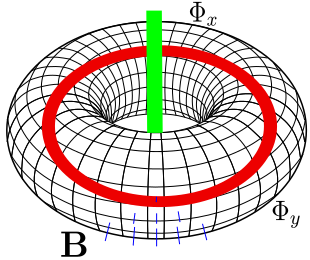
\includegraphics[scale=0.3]{Simple_Torus.png}
\end{figure}

Add two magnetic flux: $A_x = \frac{\Phi_x}{L_x} \quad A_y = \frac{\Phi_y}{L_y} + Bx$.

\end{center}
\end{frame}


\begin{frame}
\frametitle{Thoulesse picture}
\begin{center}

\[
\Delta \mathcal{H} = - \frac{J_x \delta \Phi_x}{L_x} - \frac{J_y \delta \Phi_y}{L_y}
\]

\textbf{Hypothesis}: the ground state $\ket{\psi_0} = \ket{\psi_{\Phi_x, \Phi_y}}$ is non degenerate $\forall \Phi_x, \Phi_y$.

\[
\delta \ket{\psi_0} = \ket{\psi_0} + \sum_{n \neq 0} \frac{\bra{n} \Delta \mathcal{H} \ket{\psi_0}}{E_n - E_0} \ket{n}
\]

\[
\frac{\partial \ket{\psi_0}}{\partial \Phi_i} = \sum_{n \neq 0} \frac{\bra{n} \Delta J_i \ket{\psi_0}}{E_n - E_0} \ket{n} 
\]

%TODO è sufficience richiede che non ci sia degenrazione del ground state? Non serve un gap? Studiare se serve il gap. Per invalidare l'argomento comunque basta un degenrazione del ground state del qauntum hall sul toro.

By using the Kubo formula for linear reponse
\[
\sigma_{xy} = i \hbar \left( \frac{\partial}{\partial \Phi_y}  \bra{\psi_0} \frac{\partial \ket{\psi_0}}{\partial \Phi_x} - \frac{\partial}{\partial \Phi_x} \bra{\psi_0} \frac{\partial \ket{\psi_0}}{\partial \Phi_y} \right)
\]
 
\end{center}
\end{frame}


\begin{frame}
\frametitle{Thoulesse picture}
\begin{center}

%Quando inserisco un intero flusso l'Hamiltoniana rimane la stessa a meno di tarsformazioni di gauge. Anche lo spettro fa la stessa cosa. Quindi le funzioni d'onda dopo l'insersezione adiabatica sono le stesse a meno di una funzione dell'angolo \phi. La connessione A è esattamente la stessa e si può quindi pensare che sia periodica nelle variabili di fluso. Realizzando quindi la geometria toroidale. 

Spiegare perché si possono considerare $\Phi$ come coordinate periodiche (avendo come spazio di base un toro) e finire il discorso.... A a che fare con le condizioni al bordo periodiche.

\[
\mathcal{A} = 
\]

%TODO Giutificare!! Si può fare!
\textbf{Hypothesis}: the conductance is indipendent of $\Phi_x$ and $\Phi_y$, thus we can average over this variables:

\end{center}
\end{frame}


\begin{frame}
\frametitle{TKNN invariant}
\begin{center}

This thing i don't talk
Però cercare di giustificare perché il numero di Chern deve essere quantizzato.

\end{center}
\end{frame}

\begin{frame}
\frametitle{Chiral edge modes}
\begin{center}

Neither this thing

\end{center}
\end{frame}

\begin{frame}
\frametitle{Limits of the previous formulations}
\begin{center}

\textbf{All this explainations somehow are based on a set of seemingly unjustified assumption!}

\vspace{20pt}

Later works somehow places this effect of a more rigorous basis.

\end{center}
\end{frame}

\end{comment}

\begin{frame}
\frametitle{Fractional Quantum Hall Effect}
\begin{center}

In 1982 Stormer and Tsui discover fractional conductance plateau.

\begin{figure}[!htb]
\centering
\includegraphics[scale=0.25]{fractional.png}
\end{figure}

\end{center}
\end{frame}

\begin{frame}
\frametitle{Fractional Quantum Hall Effect}
\begin{center}

\begin{itemize}

\item The FQHE should be associated to a fractional filling of the Landau level.

\item For an interacting problem it doesn't makes sense to talk about Landau levels occupancy since there will be no more single particle eigenstates.

%Laughlin nobel lecture: The L. S. cannot be adiabatically connected with a state where the elctrons are non interacting.
%WHY??
\item We cannot treat the interaction perturbatively, nonetheless we assume the ground state wavefunction to be in the Lowest Landau Level (we again ignore level mixing).
\end{itemize}
\[
\psi = f(z) e^{-\sum_{i} \frac{|z_i|^2}{4 l_B^2}} 
\]
where $z$ is the set of all the coordinates of the electrons and $f(z)$ is an \textbf{holomorphic} function.

%We expect each  Landau level to evolve a number of gaps due to the interactions between electrons. Adding disorder ($V \ll E_{int}$) induces a localization of states for each band. \textbf{Can we adapt the pumping argument?}

%...
%AGGIUNGERE UN AIMMAGINE DELLA MOLTIPLICAZIONE DEI GAP - Queste %immagini non hanno senso perché lo spettro di singola particella non %ha più senso.

\end{center}
\end{frame}

\begin{frame}
\frametitle{The Vandermonde determinant}
\begin{center}

The Slater determinant for a completely filled Landau level is:

\[
\det \begin{pmatrix} 1&1&\cdots & 1 &1\\z_1&z_2&\cdots &z_{n-1}&z_{n}\\\vdots&\vdots&\ddots&\vdots&\vdots\\z_1^{n-2}&z_2^{n-2}&\cdots&z_{n-1}^{n-2}& z_{n}^{n-2}\\z_1^{n-1}&z_2^{n-1}&\cdots&z_{n-1}^{n-1}&z_{n-1}^{n}\end{pmatrix} = \prod_{i < j} \left( z_i - z_j \right)
\]
with the addictional exponential factor the state becomes:
\[
\psi \left( z \right) = \prod_{i < j} \left( z_i - z_j \right) e^{-\sum_{i} \frac{| z_i |^2}{4 l_B^2}}
\]

\end{center}
\end{frame}

\begin{frame}
\frametitle{Laughlin ansatz}
\begin{center}

%lo spazio di Hilber è definito dallo span di queste funzioni d'onda che indichiamo come funzioni d'onda di un certo livello di landau. Anche dopo che aggiungo l'interazione lo spazio di Hilbert è sempre quello e gli autostati sono combinazioni lineari di quelli liberi (ci sta una matrice unitaria che collega le due basi ortonormali) e quindi il numero di stati totali è lo stesso. La funizione d'onda li Laughlin contengono stati che per appartenere allo spazio di Hilbert devono vivere su un area abbastanza grande e quindi l'equivalente problema libero deve essere a una filling fraction. E' chiaro altresì che non ha senso parlare di ocupazione quando ho interazione.

Laughlin proposed the following wave function to account for the plateau at filling fraction $\nu = \frac{1}{m}$:

\[
\psi \left( z \right) = \prod_{i < j} \left( z_i - z_j \right)^m e^{-\sum_{i} \frac{| z_i |^2}{4 l_B^2}}
\]

$m = 2k + 1$ because of the Pauli exclusion principle.

The maximum power of $z_1$ is $m (N-1) \sim m N$ thus the area of the sample  is $A = 2 \pi m N l_B^2$ thus the total number of states is $mN$ and $\nu = \frac{N}{m N} = \frac{1}{m}$.

What does it mean to have a fractional filling \textbf{when single particle states don't make} sense anymore?


%In un campione di una certa area saremmo portati a interpretare questo risultato come se per bassi numero di occupazione gli elettroni fossero vicini al centro e per alti numri di occupazione essi arrivassero fino ai bordi del campione: è vero questo???

%ATTENZIONE BENE: Non ha senso parlare di stati di singola particella quando ho interazione. Tuttavia possiamo pensare che gli stati non interagenti definiscano l'Hilbert space. Poi non bisogna far altro che diagonalizzare l'interazione di Coloumb sul lowest landau level di stati multiparticella ottenuti mettendo insieme un certo numero di elettroni che riempono sono in maniera partiale un landau level. In effetti ho più di uno di questi stati proprio perché non sto considerando il sistema come pieneo. Sennò ne avrei uno solo (tutti gli elettroni che occupano tutti gli m antisimmetrizati). Invece ne ho di più che si mescolano. Il ragioanmento di sopra mi dice che nelle funzioni c'onda mescolate che costituiscono l'ansatz di laughlin l'esponente in z delle funzioni d'onda elettroniche ci da informazioni sull'area del sample e ci dice che è mN. Cieò questa componente nella funzione d'onda interagente può essere comparsa solamnte se il sistema possedeva uno stato a singola particelle che si estendeva fino a quel raggio e questo è di fatto solo possibile se l'area del campione è abbastanza grande. questo significa avere un fractional filling.

\end{center}
\end{frame}

\begin{frame}
\frametitle{Laughlin ansatz}
\begin{center}

Pair correlation functions for $m = 3$ and $m=5$:

\begin{figure}[!htb]
\centering
\includegraphics[scale=0.2]{gfunction.png}
\end{figure}

%Why can it be considered like a liquid? The g(r) has the typical behaviour of a liquid: it goes to one in the asymptotic limit instead of becoming periodic (tis is the case of a solid)

The Laughlin ansatz effectively keeps the electron apart lowering the Coloumb interaction energy. It's a \textbf{liquid phase} of the electron fluid, there is also a competing solid phase: the \textbf{Wigner crystal}.

\end{center}
\end{frame}

\begin{frame}
\begin{center}

Comparison of a random distribution of electrons (left) and one following the Laughlin ansatz (right). Density fluctuations are \textbf{suppressed}.

\begin{figure}[!htb]
\centering
\includegraphics[scale=0.4]{comparison.png}
\end{figure}

\end{center}
\end{frame}


\begin{frame}
\frametitle{The plasma analogy}
\begin{center}

We can shed light on the Laughlin ansatz by exploiting the analogy with a classical plasma:

\[
\hat{n}(z) = \sum_i \delta (z - z_i)
\]

\[
n(z) = \bra{\psi} n(z) \ket{\psi} = \frac{\int \prod_{i=1}^{N} d^2 z_i n(z) P \left[ z \right] }{ \int \prod_{i=1}^{N} d^2 z_i P \left[ z \right]}
\]

\[
P \left[ z \right] = \prod_{i < j} \frac{|z_i - z_j|^{2m}}{l_B^{2m}} e^{-\sum_{i} \frac{| z_i |^2}{2 l_B^2}}
\]

\end{center}
\end{frame}

\begin{frame}
\frametitle{The plasma analogy}
\begin{center}

Particles of charge $-m$ inteacting with a uniform background

\[
P \left[ z \right] = e^{- \beta U(z)}
\]
\[
U(z) = - m^2 \sum_{i < j} \log \left( \frac{| z_i - z_j|}{l_B} \right) + \frac{m}{4 l_B^2} \sum_{i = 1}^{N} |z_i|^2 \quad \beta = \frac{2}{m}
\]

%TODO CONTROLLARE I SEGNI


Background charge density: $\rho_0 = -\frac{1}{2 \pi l_B^2}$. 

%TODO (find a way to argue the filling fractiona is still meningful) 
The plasma is globally neutral. At filling fraction the background charge is screened with a uniform density.
\[
n = \frac{1}{2 \pi l_B^2 m}
\]

%Dire che il fluido di elettroni è ul liquido per m piccoli (cioè temperature alte...), il passaggio dal fatto che il modello statistico desciva un fluido al fatto che lo descriva la funzione di Lughlin non è in effetti scontato (ma lo facciamo lo stesso...)

\end{center}
\end{frame}

\begin{frame}
\frametitle{Quasiholes}
\begin{center}
We excite the Laughlin vacuum by adding a ``vortex" at position $\eta$:

\[
\psi \left( z ; \eta \right) = \prod_{i = 1}^N \left( z_i - \eta \right) \prod_{i < j} \left( z_i - z_j \right)^m e^{-\sum_{i} \frac{| z_i |^2}{4 l_B^2}}
\]

Charge depletion aroud $\eta$ (quasihole). Carries a fractional charge $e^{*} = \frac{e}{m}$.

In the plasma analogy it behaves like an impurity of charge $q = -1$:
\[
U(z) = - m^2 \sum_{i < j} \log \left( \frac{| z_i - z_j|}{l_B} \right) - m \sum_{i = 1}^{N} \log \left( \frac{| z_i - \eta|}{l_B} \right) + \frac{m}{4 l_B^2} \sum_{i = 1}^{N} |z_i|^2 
\]

%The interaction of the impurity with the background is missing ...
There is something strange with this potential...

\end{center}
\end{frame}

%When doing tis kind of excitations we are not actually adding charge to the system as the total number of electrons doesn't change (we are just reshaping a bit the charge distribution to crate a valley).

\begin{comment}
\begin{frame}
\frametitle{Quasiholes}
\begin{center}
An actual picture of quasi-holes (with different charges) from Yang-Le Wu, B. Estienne, N. Regnault, and B. Andrei Bernevig (2014)

%TODO: Dire quanto sono grandi questi quasihole...
\begin{figure}[!htb]
\centering
\includegraphics[scale=0.2]{quasiholes.png}
\end{figure}

\end{center}
\end{frame}
\end{comment}

\begin{comment}
\begin{frame}
\frametitle{Haldane pseudopotential}
\begin{center}
We can see that the excitaions must be gapped (TODO)

Inserisco questa parte e dico che la funzione d'onda di Laughlin è un autostato esatto ell'Hamiltoniana di Haldane e questo può aiutare a giustificare il pumping argument? Secondo me no.

\end{center}
\end{frame}
\end{comment}

\begin{frame}
\frametitle{Quasiparticles}
\begin{center}
Excitations that carry a charge $e^{*} = -\frac{e}{m}$. We need to increas the local density of the electrons, thus diminuish the relative angular momentum of a pair of particles. We cannot divide by $z$ (analiticy!).

\[
\psi = \left[ \prod_{i=1}^{N} \left( 2 \frac{\partial}{\partial z_i} - \bar{\eta} \right) \prod_{k < l} ( z_k - z_l ) ^m \right] e^{- \sum_{i = 1}^{n} \frac{|z_i|^2}{4 l_B^2}}
\]

\end{center}
\end{frame}

\begin{frame}
\frametitle{Experimental proof of fractionalization}
\begin{center}


R. de-Picciotto, M. Reznikov, M. Heiblum, V. Umansky,
G. Bunin, and D. Mahalu, “Direct observation of a fractional charge”, Nature 389, 162 (1997).

%TODO : what happens when the filling fraction is not an integer??? How the flux get redistributed?? What does it mean if one adds an electron it will split??


\begin{minipage}[t]{0.60\linewidth}
\begin{figure}[!htb]
\centering
\includegraphics[scale=0.20]{shotnoise.png}
\end{figure}
\end{minipage}\hfill
\begin{minipage}[t]{0.40\linewidth}
\begin{figure}[!htb]
\centering
\includegraphics[scale=0.3]{backscatter.png}
\end{figure}
\end{minipage}

\end{center}
\end{frame}

\begin{frame}
\frametitle{Collective excitations}
\begin{center}

A systematic study of the collective excitations involves taking the immaginary part of the density-density response function $\chi_{nn}(\mathbf{q}, \omega)$. 

\begin{figure}[!htb]
\centering
\includegraphics[scale=0.25]{neutral.png}
\end{figure}
S. M. Girvin, 1998. Excitations are \textbf{gapped}. The liquid is incompressible by definition. Ansatz wavefunction for those excitations (similar to the one by Feynman for superfluids).

\end{center}
\end{frame}

\begin{comment}
\begin{frame}
\frametitle{Collective excitations}
\begin{center}

:

projected density operators...

\end{center}
\end{frame}
\end{comment}

%TODO Togliere questo pumping argment che non so giustificare
\begin{frame}
\frametitle{Laughlin flux insertion}
\begin{center}

%TODO: I suspect you cannot link adiabattically the ground state of the non interacting liuid with the one of the interacting liquid. Indeed.

What is the state after the adiabatic flux insertion if it starts as $\psi$?

If we perform a singular gauge transformation on $\psi$ to insert a flux in the origin we have:

\begin{figure}[!htb]
\centering
\includegraphics[scale=0.3]{fluxInsertion.png}
\end{figure}

$\mathbf{A} = Arg \left( z \right)$ is precisely a vortex with $\mathbf{B} = 0$ field and a singularity in the origin.

\[
\psi^{'}(z) = \prod \frac{z_i}{|z_i|} \psi(z)
\]

\end{center}
\end{frame}

\begin{frame}
\begin{center}

This is obviously not in the LLL so Laughlin proposed that the adiabatic evolution would have led to:

\[
\psi^{'}(z) = \prod z_i \prod_{i<j} (z_i - z_j)^m e^{- \sum_{i} \frac{|z_i|^2}{4 l_B^2}}
\]

This is consistent with the fact that starting from an eigenstate if there is no level crossing I get in another eigenstate.


A quasihole deplets a charge $\frac{e}{m}$ from its centers, this must have flown through the boundaries and we get $\sigma_{xy} = \frac{e^2}{h} \frac{1}{m}$.

\vspace{10pt}
A similar argument goes through in presence of disorder.

\end{center}
\end{frame}

%Evito la pipa sugli anioni forse è meglio

\begin{comment}
\begin{frame}
\frametitle{Particles in 3D}
\begin{center}

We imagine exchanging two identical particles. 
In 3D the path of two particle exchanging position can be continously deformed to doing no exchange. 

\[
\psi (\mathbf{r_1}, \mathbf{r_2}) \rightarrow e^{i \alpha} \psi (\mathbf{r_2}, \mathbf{r_1}) \rightarrow e^{2 i \alpha} \psi (\mathbf{r_1}, \mathbf{r_2}) = \psi (\mathbf{r_1}, \mathbf{r_2})
\]

thus $e^{i \alpha} = \pm 1$. 

INSERIRE IMMAGINE SFERA


\end{center}
\end{frame}

\begin{frame}
\frametitle{Anyons in 2D}
\begin{center}
In 2D this is no longer true.

INSERIRE IMMAGINE


\end{center}
\end{frame}
\end{comment}

\begin{frame}
\begin{center}

\Large{Thanks for your attention}

\end{center}
\end{frame}

\begin{frame}
\frametitle{Berry phase}
\begin{center}

Consider a state of $M$ quasiholes:

\[
\braket{z, \bar{z} | \eta_1, \eta_2, .., \eta_M} = \frac{1}{Z}\prod_{j = 1}^{M} \prod_{i = 1}^{N} ( z_i - \eta_j ) \prod_{k < l} \left( z_k - z_l \right)^{m} e^{- \sum_{i} \frac{|z_i|^2}{4 l_B^2}}
\]

\[
Z = \int \prod d^2 z_i \exp \left( \sum_{i < j} \log | z_i - \eta_j|^2 + m \sum_{k, l} \log |z_k - z_l|^2 - \frac{1}{2 l_B^2} |z_i|^2 \right)
\]

What happens if we slowly exchange two quasiparticles? If they are indistinguishable particles the wavefunction stay the same up to a Berry phase.

\end{center}
\end{frame}

\begin{frame}
\frametitle{Berry phase}
\begin{center}

Let's compute the Berry phase:

\[
\mathcal{A}_{\mathbf{\eta}} = - i \bra{\mathbf{\eta}} \frac{\partial}{\partial \eta} \ket{\mathbf{\eta}} = -\frac{i}{2} \frac{\partial \log Z}{\partial \eta} \quad \mathcal{A}_{\bar{\eta}} = +\frac{i}{2} \frac{\partial \log Z}{\partial \bar{\eta}}
\]

We use again the plasma analogy!

%$Z$ is the partition function of a plasma of particles of charge $m$ with impurities of charge $1$. The leading mechanis here is screening and the free energy is insensitive on the position of the impurities.

We add the interaction of the impurities between themselves and with the background. The correct internal energy should be:
\[
U(z_k; \eta_i) =  - m \sum_{k < l} \log | z_i - \eta_j|^2 - m^2 \sum_{k, l} \log |z_k - z_l|^2 - \frac{1}{2 l_B^2} |z_i|^2 +
\]
\[
-\sum_{i < j} \log | \eta_i - \eta_j| + \frac{m}{4 l_B^2} \sum_k |z_k|^2 + \frac{1}{4 l_B^2} \sum_i |\eta_i|^2
\]

\end{center}
\end{frame}

\begin{frame}
\frametitle{Berry phase}
\begin{center}

The correct partition function is thus:

\[
\int d^2 z_k e^{- \beta U(z_k; \eta_i)} = \exp \left( - \frac{1}{m}\sum_{i < j} \log | \eta_i - \eta_j| + \frac{1}{2 m l_B^2} \sum_i |\eta_i|^2 \right) Z
\]

As long as the plasma is the liquid phase (which is for $m < 70$) because of the screening the partition function should be independent on the position of the impurities $\eta_i$, thus we get:

\[
Z = C \exp \left( \frac{1}{m}\sum_{i < j} \log | \eta_i - \eta_j| - \frac{1}{2 m l_B^2} \sum_i |\eta_i|^2 \right)
\]

\end{center}
\end{frame}

\begin{frame}
\frametitle{Berry phase}
\begin{center}
The Berry phase becomes:

\[
\mathcal{A}_{\eta} = - \frac{i}{2 m} \sum_{i \neq j} \frac{1}{\eta_i - \eta_j} + \frac{i \bar{\eta}_i}{4 m l_B^2} 
\]

and a similar expression for the anti-holonomic connection.

They holds if the particles don't come too close to each other and break the screening approximation.

\[
\gamma = - \oint_{C} \left( \mathcal{A}_{\eta} d \eta  + \mathcal{A}_{\bar{\eta}} d \bar{\eta} \right) 
\]

\end{center}
\end{frame}

\begin{frame}
\frametitle{Charge of the quasiholes}
\begin{center}

We consider a loop of one quasihole in a region that doesn't enclose any other quasiparticle.

\[
\mathcal{A}_{\eta} = \frac{i \bar{\eta}}{4 m l_B^2}
\quad
\mathcal{A}_{\bar{\eta}} = \frac{-i \eta}{4 m l_B^2}
\]

\[
\gamma = \frac{e \Psi}{m \hbar}
\]

It's the Arhanov-Bohm phase of a particle of charge $\frac{e}{m}$.

\end{center}
\end{frame}


\begin{frame}
\frametitle{Fractional statistics}
\begin{center}
We generate two quasiparticles at $\eta_1$ and $\eta_2$. We take $\eta_1$ on a journey that encloses $\eta_2$.

We neglet the Arhaniv-Bohm phase and get:

\[
\gamma = - \frac{1}{2 m} \left( \oint \frac{d \eta_1}{\eta_1 - \eta_2} + \oint \frac{d \bar{\eta_1}}{\bar{\eta}_1 - \bar{\eta}_2} \right) = \frac{2 \pi i}{m}
\]

Quasiholes (and quasiparticles) are nor fermions or bosons. Upon the exchange of two of them the wavefunction gets a phase of $\frac{2 \pi i}{m}$. These particles are called \textbf{anyons}.


\end{center}
\end{frame}


\begin{comment}

%TUTTO DA QUI IN POI NON METTERE

\begin{frame}
\frametitle{Topological degeneracy}
\begin{center}


\end{center}
\end{frame}

\begin{frame}
\frametitle{Other filling fractions}
\begin{center}

We consider each vortex $\left( z - \eta \right)$ as linked to a true electron.

\textbf{Composite fermion}: electron with $m$ vortex sticked to it.

\begin{figure}[!htb]
\centering
\includegraphics[scale=0.5]{composite.png}
\end{figure}

\end{center}
\end{frame}

\begin{frame}
\frametitle{Composite fermions}
\begin{center}

Let's see what happens if we exchange two of them:

\end{center}
\end{frame}

\begin{frame}
\frametitle{Composite fermions}
\begin{center}


\end{center}
\end{frame}

\begin{frame}
\frametitle{Half filled Landau level}
\begin{center}


\end{center}
\end{frame}



\begin{frame}
\frametitle{Landau liquid}
\begin{center}


\end{center}
\end{frame}

\begin{frame}
\frametitle{Moore-Read State}
\begin{center}


\end{center}
\end{frame}

\begin{frame}
\frametitle{Non-Abelian anyons}
\begin{center}


\end{center}
\end{frame}
\end{comment}
%----------------------------------------------------------------------------------------

\end{document} 